\documentclass[a4paper,12pt]{article}
\usepackage{graphicx}
\usepackage[dvipsnames]{xcolor}
\usepackage{wrapfig}
\usepackage{color}
\usepackage{graphicx}
\usepackage{subfigure}
\usepackage{multirow}
\usepackage[section]{placeins}
\usepackage{tikz}
\usepackage{framed}
\usetikzlibrary{automata,positioning,arrows,positioning}
\usepackage{amsmath}
\usetikzlibrary{matrix,calc}
\usetikzlibrary{positioning}
\usetikzlibrary{matrix}
\usepackage{alltt}
\usepackage{etoolbox}
\pgfdeclarelayer{background}
\pgfsetlayers{background,main}
\usepackage[hidelinks]{hyperref}
\usepackage[nottoc]{tocbibind}
\definecolor{darkred}{rgb}{0,0,0.5}
\definecolor{darkgreen}{rgb}{0,0.5,0}
\definecolor{darkblue}{rgb}{0.5,0,0}
\hypersetup{ colorlinks, linkcolor=darkblue, filecolor=darkgreen, urlcolor=darkred, citecolor=darkblue}

\begin{document}
\begin{titlepage}
\begin{center}
	\textsc{\LARGE Indian Institute of Technology
			\\Bombay} \\[2.5cm]
	\begin{figure}[ht!]
	\begin{center}
		\includegraphics[scale = 0.6]{images/1}
	\end{center}
	\end{figure}

    \vspace*{-0.6cm}
	\hrule \hrule \hrule
	\vspace{0.5cm}
	\textsc{\Large CS 490 :RnD Project}\\[0.5cm]
	% Title
	{\huge \bfseries Dynamic Server Consolidation Problem (DSCP)} \\[0.5cm]
	\hrule \hrule \hrule
	\vspace{4cm}

	% Author and supervisor
	\begin{minipage}{0.5\textwidth}
	\begin{flushleft} \large
		\emph{By:} \\
		Aman Mangal (100050015) \\
		Amit Panghal (100050016)
	\end{flushleft}
	\end{minipage}
	\begin{minipage}{0.4\textwidth}
	\begin{flushright} \large
		\emph{Coordinator:} \\
		Prof. Varsha Apte
	\end{flushright}
	\end{minipage}
	\vspace{1cm}

	% Bottom of the page
	{\large \today}
\end{center}
\end{titlepage}
\tableofcontents
\vspace{0.5cm}
\hrule \hrule \hrule
\newpage

\section{Introduction}
Dynamic Server Consolidation (DSCP) is a technique used in data centers in order to maximize profit by reducing resource utilization specifically, number of physical machines to host a given set of virtual machines. Live Migration \cite{live_migration} allows moving virtual machines from one physical machine to other, without utilizing much of computing resources in real time. This makes DSC more interesting and introduces possibility of further optimization. By consolidating virtual machines more compactly on least number of physical machines, predicting future workload and re-configuring VM-to-PM placement in realtime leads to minimal cost for a data center to host same number of applications.

In general, finding the optimal VM-to-PM placement is an NP hard problem since it can be reduced to a knapsack problem. Various heuristics have been proposed to achieve close to optimal solutions. In \cite{ieee_mdp}, DSC problem is formulated as Markov Decision Process (MDP) to find the optimal solution. It also proposes a profit based approach in order to evaluate such heuristics. In this report, we solve the problem using shortest path algorithms. We first prove that the shortest path algorithms are applicable and can be used to solve the MDP \footnote{From now onward, MDP refers to our formulation of DSCP as MDP unless
specified explicitly} with slight modification and then present the results.

\section{Existing Work}
Previous work presented in \cite{ieee_mdp} has taken a different approach towards solving DSCP compared to solving it as bin packing problem. It has following main contributions-
\begin{enumerate}
\item The paper proposed a utilization based profit model for a data center. The model takes into account migration cost, SLA penalty and power cost. It is resilient to change in technology in the sense that it quantifies each cost and evaluates a final total cost. Such a quantity can be used to compare various algorithms proposed to reduce cost of the data center providing Infrastructure as a Service (IaaS).
\item It formulates the cyclic workload DSC problem as finite horizon MDP. Backward induction method proposed by Puterman is used to find an optimal solution which is then compared to khanna \cite{khanna} to show the global optimality of MDP.
\end{enumerate}

Such an approach quickly suffers from the "curse of dimensionality" due to very large number of MDP states. In this report, we approach the same MDP problem from the perspective of finding shortest path and propose heuristics to find an optimal solution in least possible time.

\section{Shortest Path Algorithms}
In graph theory, the shortest path problem is the problem of finding a path between two vertices (or nodes) in a graph such that the sum of the weights of its constituent edges is minimized. There are following constraints while using these algorithms to solve MDP-
\begin{itemize}
\item MDP is a profit based model which tries to maximize the profit whereas shortest path algorithms minimizes the total path cost.
\item MDP may have negative edges. Some of the shortest path algorithms may not be valid in the presence of a negative edge
\end{itemize}

In the next section, we slightly modify the MDP in order to be able to apply shortest path algorithms to find the optimal path.

\subsection{Applicability}
We propose following modifications in the original MDP formulation to be able to use any shortest path algorithm to find maximum profit-

\begin{figure}[h]
\centering
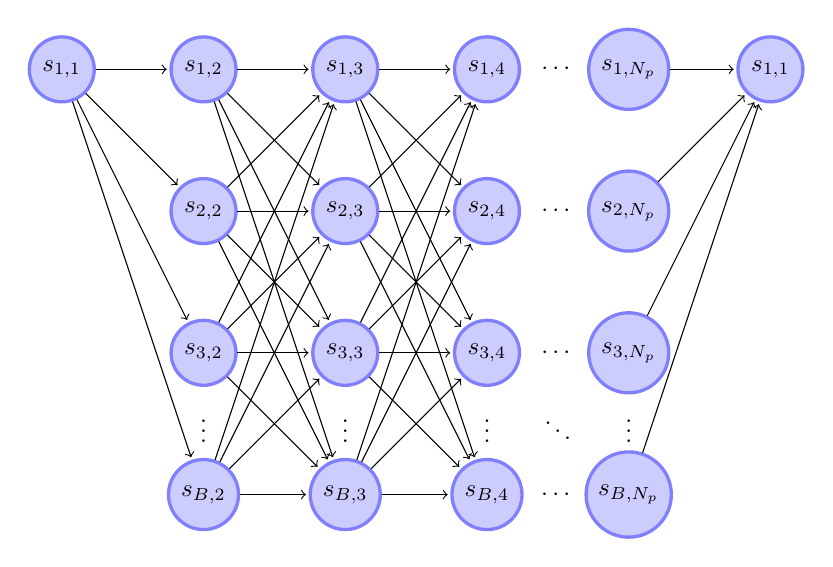
\begin{tikzpicture}[scale=0.9, transform shape, shorten >=1pt, node distance=2cm,auto]
\tikzstyle{every state}=[>=stealth', draw=blue!50, very thick, fill=blue!20]
\node[state] (s11)                {$s_{1,1}$};
\node[state] (s12) [right of=s11] {$s_{1,2}$};
\node[state] (s22) [below of=s12] {$s_{2,2}$};
\node[state] (s32) [below of=s22] {$s_{3,2}$};
\node[state] (s13) [right of=s12] {$s_{1,3}$};
\node[state] (s23) [below of=s13] {$s_{2,3}$};
\node[state] (s33) [below of=s23] {$s_{3,3}$};
\node[state] (s14) [right of=s13] {$s_{1,4}$};
\node[state] (s24) [below of=s14] {$s_{2,4}$};
\node[state] (s34) [below of=s24] {$s_{3,4}$};

\tikzstyle{every state}=[>=stealth', draw=none, very thick, node distance=1cm]
\node[state] (sd2) [below of=s32] {$\vdots$};
\node[state] (sd3) [below of=s33] {$\vdots$};
\node[state] (sd4) [below of=s34] {$\vdots$};

\node[state] (s1d) [right of=s14] {$\cdots$};
\node[state] (s2d) [right of=s24] {$\cdots$};
\node[state] (s3d) [right of=s34] {$\cdots$};
\node[state] (sdd) [right of=sd4] {$\ddots$};
\node[state] (sdn) [below of=sdd] {$\cdots$};

\node[state] (snd) [right of=sdd] {$\vdots$};

\tikzstyle{every state}=[>=stealth', draw=blue!50, very thick, fill=blue!20, node distance=1cm, auto]
\node[state] (sn2) [below of=sd2] {$s_{B,2}$};
\node[state] (sn3) [below of=sd3] {$s_{B,3}$};
\node[state] (sn4) [below of=sd4] {$s_{B,4}$};

\node[state] (s1n) [right of=s1d] {$s_{1,N_p}$};
\node[state] (s2n) [right of=s2d] {$s_{2,N_p}$};
\node[state] (s3n) [right of=s3d] {$s_{3,N_p}$};
\node[state] (snn) [right of=sdn] {$s_{B,N_p}$};

\tikzstyle{every state}=[>=stealth', draw=blue!50, very thick, fill=blue!20, node distance=2cm, auto]
\node[state] (s11') [right of=s1n] {$s_{1,1}$};

\foreach \x in {s12, s22, s32, sn2}
{\path[->] (s11) edge node {} (\x);}
\foreach \x in {s12, s22, s32, sn2}
{\path[->] (\x) edge node {} (s13)
                edge node {} (s23)
                edge node {} (s33)
                edge node {} (sn3);}
\foreach \x in {s13, s23, s33, sn3}
{\path[->] (\x) edge node {} (s14)
                edge node {} (s24)
                edge node {} (s34)
                edge node {} (sn4);}
\foreach \x in {s1n, s2n, s3n, snn}
{\path[->] (\x) edge node {} (s11');}
\end{tikzpicture}
\caption{MDP formulation}
\end{figure}

\begin{enumerate}
\item Multiply each edge weight with -1 to convert them into cost
\item Shift (add or subtract) each edge weight by a constant value such that all edge weights in MDP are positive.
\end{enumerate}

Now we prove that the MDP thus constructed has the same optimal path as the original MDP. Consider 2 MDPs, MDP B in Figure \ref{fig:B} having weights shifted by a fixed offset than the MDP A in Figure \ref{fig:A}, such that all the weights are positive in MDP B. We prove by contradiction as follows-

\begin{itemize}
\item Assuming only one optimal path in MDP A
\item Let's say optimal paths in both the MDPs are different, $P_A$ and $P_B$
\item Cost of $P_A$, in MDP B-\\
\hspace*{1cm} $CB_{P_A}$ = ($CA_{P_A}$ + $N_p$*offset ) \\
\hspace*{3cm} where CX: Cost in MDP X, $N_p$: Number of phases
\item Cost of optimal path of MDP B, in MDP B-\\
\hspace*{1cm} $CB_{P_B}$ = ($CA_{P_B}$ + $N_p$*offset)
\item Clearly, $CA_{P_A} \leq CA_{P_B}  \Rightarrow  CB_{P_A} \leq CB_{P_B}$
\item But we assumed $P_B$ as optimal and only path in MDP B. $P_A$ cannot be more optimal than $P_B$. This leads to a contradiction
\item Proof can be extended to MDPs having more than one optimal path
\end{itemize}

\begin{figure}[h]
\begin{minipage}{.49\textwidth}
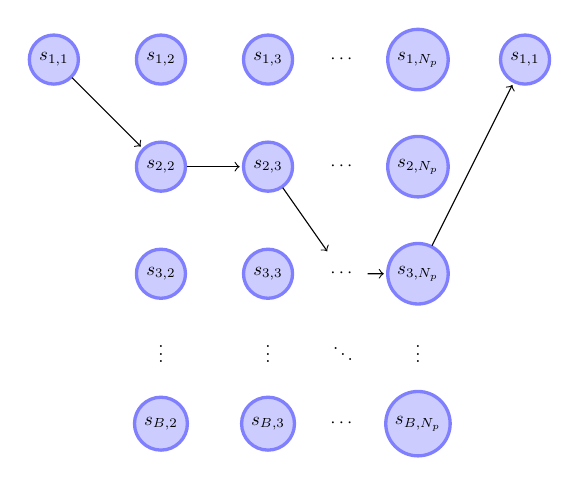
\begin{tikzpicture}[scale=0.68, transform shape, shorten >=1pt, node distance=2cm,auto]
\tikzstyle{every state}=[>=stealth', draw=blue!50, very thick, fill=blue!20]
\node[state] (s11)                {$s_{1,1}$};
\node[state] (s12) [right of=s11] {$s_{1,2}$};
\node[state] (s22) [below of=s12] {$s_{2,2}$};
\node[state] (s32) [below of=s22] {$s_{3,2}$};
\node[state] (s13) [right of=s12] {$s_{1,3}$};
\node[state] (s23) [below of=s13] {$s_{2,3}$};
\node[state] (s33) [below of=s23] {$s_{3,3}$};

\tikzstyle{every state}=[>=stealth', draw=none, very thick, node distance=1.4cm]
\node[state] (sd2) [below of=s32] {$\vdots$};
\node[state] (sd3) [below of=s33] {$\vdots$};

\node[state] (s1d) [right of=s13] {$\cdots$};
\node[state] (s2d) [right of=s23] {$\cdots$};
\node[state] (s3d) [right of=s33] {$\cdots$};
\node[state] (sdd) [right of=sd3] {$\ddots$};
\node[state] (sdn) [below of=sdd] {$\cdots$};

\node[state] (snd) [right of=sdd] {$\vdots$};

\tikzstyle{every state}=[>=stealth', draw=blue!50, very thick, fill=blue!20, node distance=1.4cm, auto]
\node[state] (sn2) [below of=sd2] {$s_{B,2}$};
\node[state] (sn3) [below of=sd3] {$s_{B,3}$};

\node[state] (s1n) [right of=s1d] {$s_{1,N_p}$};
\node[state] (s2n) [right of=s2d] {$s_{2,N_p}$};
\node[state] (s3n) [right of=s3d] {$s_{3,N_p}$};
\node[state] (snn) [right of=sdn] {$s_{B,N_p}$};

\tikzstyle{every state}=[>=stealth', draw=blue!50, very thick, fill=blue!20, node distance=2cm, auto]
\node[state] (s11') [right of=s1n] {$s_{1,1}$};

\path[->] (s11) edge node {} (s22);
\path[->] (s22) edge node {} (s23);
\path[->] (s23) edge node {} (s3d);
\path[->] (s3d) edge node {} (s3n);
\path[->] (s3n) edge node {} (s11');
\end{tikzpicture}
\caption{(A)\label{fig:A}}
\end{minipage}
\vrule{}
\begin{minipage}{0.5\textwidth}
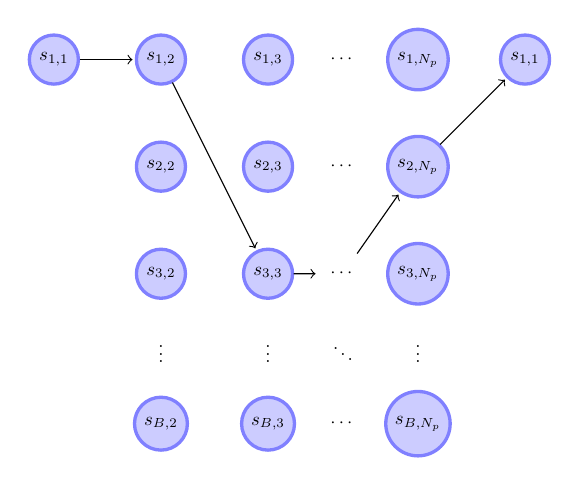
\begin{tikzpicture}[scale=0.68, transform shape, shorten >=1pt, node distance=2cm,auto]
\tikzstyle{every state}=[>=stealth', draw=blue!50, very thick, fill=blue!20]
\node[state] (s11)                {$s_{1,1}$};
\node[state] (s12) [right of=s11] {$s_{1,2}$};
\node[state] (s22) [below of=s12] {$s_{2,2}$};
\node[state] (s32) [below of=s22] {$s_{3,2}$};
\node[state] (s13) [right of=s12] {$s_{1,3}$};
\node[state] (s23) [below of=s13] {$s_{2,3}$};
\node[state] (s33) [below of=s23] {$s_{3,3}$};

\tikzstyle{every state}=[>=stealth', draw=none, very thick, node distance=1.4cm]
\node[state] (sd2) [below of=s32] {$\vdots$};
\node[state] (sd3) [below of=s33] {$\vdots$};

\node[state] (s1d) [right of=s13] {$\cdots$};
\node[state] (s2d) [right of=s23] {$\cdots$};
\node[state] (s3d) [right of=s33] {$\cdots$};
\node[state] (sdd) [right of=sd3] {$\ddots$};
\node[state] (sdn) [below of=sdd] {$\cdots$};

\node[state] (snd) [right of=sdd] {$\vdots$};

\tikzstyle{every state}=[>=stealth', draw=blue!50, very thick, fill=blue!20, node distance=1.4cm, auto]
\node[state] (sn2) [below of=sd2] {$s_{B,2}$};
\node[state] (sn3) [below of=sd3] {$s_{B,3}$};

\node[state] (s1n) [right of=s1d] {$s_{1,N_p}$};
\node[state] (s2n) [right of=s2d] {$s_{2,N_p}$};
\node[state] (s3n) [right of=s3d] {$s_{3,N_p}$};
\node[state] (snn) [right of=sdn] {$s_{B,N_p}$};

\tikzstyle{every state}=[>=stealth', draw=blue!50, very thick, fill=blue!20, node distance=2cm, auto]
\node[state] (s11') [right of=s1n] {$s_{1,1}$};

\path[->] (s11) edge node {} (s12);
\path[->] (s12) edge node {} (s33);
\path[->] (s33) edge node {} (s3d);
\path[->] (s3d) edge node {} (s2n);
\path[->] (s2n) edge node {} (s11');
\end{tikzpicture}
\caption{(B)\label{fig:B}}
\end{minipage}
\end{figure}

\subsection{Problem Statement}
We are given an MDP with some profit function(including negative profit values). We find cost by multiplying all profit values with -1. The cost has to be positive so that we can apply shortest path algorithms. Hence, we take an offset as one more than the minimum cost in MDP thus obtained. By subtracting offset, we get an MDP with all positive costs as edge weights. 

After solving and finding optimal path, we need to translate the cost into profit in original MDP. We add ($N_p \times$ offset) to minimum cost and multiply it with -1 to find maximum profit. Corresponding path will be the optimal path for the original MDP.

\subsection{Dijkstra's Algorithm}
This is a greedy search algorithm. It expands the node with minimum cost and try to reach to the goal node as soon as possible.

\begin{figure}[h]
\begin{framed}
\begin{alltt}
\fontsize{8pt}{10pt}\selectfont
function Dijkstra(Graph, source):
    dist[source] := 0
    for each vertex v in Graph:
        if v (not equal) source
            dist[v] := infinity
            previous[v] := undefined
        end if
        PQ.add\_with\_priority(v,dist[v])
    end for
    while PQ is not empty:
        u := PQ.extract\_min()
        for each neighbor v of u:
            alt = dist[u] + length(u, v)
            if alt < dist[v]
                dist[v] := alt
                previous[v] := u
                PQ.decrease\_priority(v,alt)
            end if
        end for
    end while
    return previous[]
\end{alltt}
\end{framed}
\vspace*{-0.6cm}
\caption{Pseudocode for Dijkstra's Algorithm}
\vspace*{-0.4cm}
\end{figure}

\subsection{A* Search}
A* is a heuristic based search. The node to be relaxed is chosen based on the minimum total cost. We already know the cost of coming to current node from source node (g value) and we guess the cost of going to goal node from current node using a heuristic (h value). The search is performed based on (f value =  g value + h value).

The node having minimum value of f (total cost) is relaxed first. Algorithm terminates when found path has, actual cost lower than the estimated cost of any path through any open node. It is guaranteed to find optimal path if heuristic is admissible. A heuristic is called \textit{Admissible} if $h(x) \leq d(x,y) + h(y) = h^*(n)$, i.e. it does not overestimate the total cost. Essentially, when the algorithm stop, admissibility makes sure that all the un-expanded nodes have higher actual total cost if calculated.

\begin{figure}[h]
\begin{framed}
\begin{alltt}
\fontsize{8pt}{10pt}\selectfont
function A*(start,goal)
    closedset := the empty set
    openset := {start}
    came\_from := the empty map
    g\_score[start] := 0
    f\_score[start] := g\_score[start] + h\_cost(start, goal)
    while openset is not empty
      current := openset node having the lowest f\_score[] value
      if current = goal
            return reconstruct\_path(came\_from, goal)
      remove current from openset and put to closedset
      for each neigh in neigh\_nodes(current)
            if neigh in closedset
              continue
            new\_g\_score := g\_score[current] + dist\_between(current,neigh)
            if neigh not in openset or new\_g\_score < g\_score[neigh]
              came\_from[neigh] := current
              g\_score[neigh] := new\_g\_score
              f\_score[neigh] := g\_score[neigh] + h\_cost(neigh, goal)
              if neigh not in openset
                    add neigh to openset
    return failure
\end{alltt}
\end{framed}
\vspace*{-0.6cm}
\caption{A* Search Algorithm}
\vspace*{-0.4cm}
\end{figure}

\subsection{Complexity Analysis}
\begin{table}[h]
\begin{tabular}{|c|c|c|}
\hline
 & \textbf{Time Complexity} & \textbf{Space Complexity} \\
\hline
Backward Induction & $N_P*B^{2}*M! + N_p*B^3$ & $N_P*B^{2}*M$ \\
\hline
Dijkstra's Algorithm & $N_P*B^{2}*M! + N_p*B^3$ & $N_p*B^2$ \\
\hline
Bellman-Ford Algorithm & $N_P*B^{2}*M! + N_p^2*B^4$ & $N_p*B^2$ \\
\hline
A* search & $N_P*B^{2}*M! + N_p*B^3$ & $N_p*B^2$ \\
\hline
\end{tabular}
\end{table}

In practice, complexity follows-
Backward Induction $>$ Dijkstra's Algorithm $>$ A* search

\section{Experimental Evaluation}
We performed test with \textit{Backward Induction}, \textit{Dijkstra's Algorithm} and \textit{A* search} and found that \textit{A* search} performs best as expected. For few number of VMs and few phases, it is possible that \textit{A*} takes more time than \textit{Backward Induction} algorithm.

For \textit{A*}, following heuristic was used. The estimated cost for a node is equal to sum of minimum costs in each phase for any state. It cut down search space and reduced the number of relaxed nodes.

\begin{table}[h]
\centering
\begin{tabular}{|c|c|c|c|}
\hline 
- & Backward Induction & Dijkstra's & A* \\ 
\hline 
Time Taken & 1234329 & 2772473 & 11471433 \\ 
\hline 
Relaxed Nodes & - & 60274 & 35712 \\ 
\hline 
\end{tabular}
\caption{5 VMs, 24 phases (random workload)}
\vspace{0.6cm}

\begin{tabular}{|c|c|c|c|}
\hline 
- & Backward Induction & Dijkstra's & A* \\ 
\hline 
Time Taken & 53138243 & 56272730 & 56558261 \\ 
\hline 
Relaxed Nodes & - & 435692 & 172501 \\ 
\hline 
\end{tabular} 
\caption{6 VMs, 12 phases (random workload)}
\vspace{0.6cm}

\begin{tabular}{|c|c|c|c|}
\hline 
- & Backward Induction & Dijkstra's & A* \\ 
\hline 
Time Taken & 1270033 & 10886275 & 11674272 \\ 
\hline 
Relaxed Nodes & - & 60143 & 1249 \\ 
\hline 
\end{tabular}
\caption{5 VMs, 24 phases (random workload, backward induction)}
\vspace{0.6cm}

\begin{tabular}{|c|c|c|c|}
\hline 
- & Backward Induction & Dijkstra's & A* \\ 
\hline 
Time Taken & 53375982 & 54879534 & 54181331 \\ 
\hline 
Relaxed Nodes & - & 432150 & 2436 \\ 
\hline 
\end{tabular}
\caption{6 VMs, 12 phases (random workload, backward induction)}
\end{table}
\vspace*{-0.5cm}

\section{Heuristic Search}
While designing heuristics, we realised that most of the cost based heuristics converge to backward induction. We, therefore, designed a non-cost based search algorithm. It searches based only on h value. h value may not necessarily be the direct cost.
It represents feasibility of state and hence likelihood of h being in the optimal path.

In a non-cost based search, we do not have any stopping criteria. We borrowed the stopping criteria from \textit{A* search}. We keep an A* based heuristic and hence f values for each node. We search based on h value but stop with the same condition as A*. Such an algorithm can have implications in a time constraint environment. If heuristic is good, \textit{Heuristic Search} may reach to the goal node early compared to \textit{A* search}.

\section{Future Work}
The following approaches to minimize the complexity to solve MDP can still be incorporated-
\begin{itemize}
\item Reduction in time of step 1
\item A* heuristics and All Pairs Algorithm \cite{Cormen}
\item Fibonacci Heap implementation
\end{itemize}

\section{Conclusion}
In this report, we tried to reduce the complexity of step 2 (Global Optimization step) in solving MDP by using shortest path algorithms. We began with proving that such algorithms are indeed applicable on the formulated MDP. We implemented \textit{Dijkstra's Algorithm}, \textit{A* search} and showed that these algorithms performs better in practice. We also saw that \textit{A* search} reduces the search space while finding the optimal path. All the code (written in C++) is available at \cite{github}.

\bibliographystyle{abbrv}
\bibliography{ref}

\end{document}
